\begin{applicationActivities}

\begin{activity}{10}
  Consider the two sets
  \begin{align*}
    S=\left\{
  \begin{bmatrix}2\\3\\1\end{bmatrix},
  \begin{bmatrix}1\\1\\4\end{bmatrix}
  \right\} & &
    T=\left\{
  \begin{bmatrix}2\\3\\1\end{bmatrix},
  \begin{bmatrix}1\\1\\4\end{bmatrix},
  \begin{bmatrix}-1\\0\\-11\end{bmatrix}
  \right\}
  \end{align*}
  Which of the following is true?

	\begin{enumerate}[(A)]
	\item \(\vspan S\) is bigger than \(\vspan T\).
	\item \(\vspan S\) and \(\vspan T\) are the same size.
	\item \(\vspan S\) is smaller than \(\vspan T\).
	\end{enumerate}

\end{activity}

\begin{definition}
  We say that a set of vectors is \term{linearly dependent} if one vector
  in the set belongs to the span of the others. Otherwise, we say the set
  is \term{linearly independent}.

  \begin{center}
  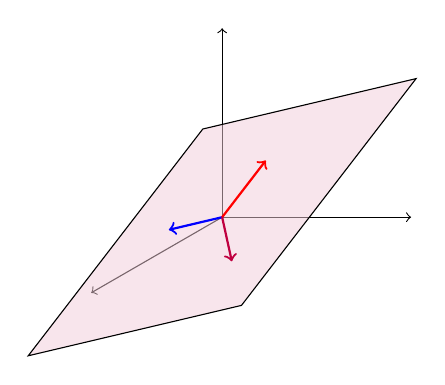
\begin{tikzpicture}[x={(210:0.8cm)}, y={(0:1cm)}, z={(90:1cm)},scale=0.4]
    \draw[->] (0,0,0) -- (6,0,0);
    \draw[->] (0,0,0) -- (0,6,0);
    \draw[->] (0,0,0) -- (0,0,6);
    \draw[fill=purple!20,fill opacity=0.5]
      (-2,-2,2) -- (6,-2,-2) -- (2,2,-2) -- (-6,2,2) -- (-2,-2,2);
    \draw[thick,blue,->] (0,0,0) -- (1,-1,0);
    \draw[thick,red,->] (0,0,0) -- (-2,0,1);
    \draw[thick,purple,->] (0,0,0) -- (1,1,-1);
  \end{tikzpicture}
  \end{center}

  You can think of linearly dependent sets as containing a redundant vector,
  in the sense that you can drop a vector out without reducing the span of the set. In the above image, all three vectors lay on the same planar subspace,
  but only two vectors are needed to span the plane, so the set is
  linearly dependent.
\end{definition}

\begin{activity}{10}
  Let \(\vect u,\vect v,\vect w\) be vectors in \(\mathbb R^n\).
  Suppose \(3\vect u-5\vect v=\vect w\), so the set
  \(\{\vect u,\vect v,\vect w\}\) is linearly dependent.
  Which of the following is true of the vector equation \(x\vect u+y\vect v+z\vect w=\vect 0\) ?
  \begin{enumerate}[(A)]
  \item It is consistent with one solution
  \item It is consistent with infinitely many solutions
  \item It is inconsistent.
  \end{enumerate}
\end{activity}

\begin{fact}
  For any vector space,
  the set \(\{\vect v_1,\dots\vect v_n\}\) is linearly dependent if and only
  if \(x_1\vect v_1+\dots+x_n\vect v_n=\vect z\) is consistent with
  infinitely many solutions.
\end{fact}

\begin{activity}{10}
  Find
  \[\RREF\begin{bmatrix}[ccccc|c]
  2&2&3&-1&4&0\\
  3&0&13&10&3&0\\
  0&0&7&7&0&0\\
  -1&3&16&14&2&0
  \end{bmatrix}
  \]
  and mark the part of the matrix that demonstrates that
  \[S=\left\{
  \begin{bmatrix}2\\3\\0\\-1\end{bmatrix},
  \begin{bmatrix}2\\0\\0\\3\end{bmatrix},
  \begin{bmatrix}3\\13\\7\\16\end{bmatrix},
  \begin{bmatrix}-1\\10\\7\\14\end{bmatrix},
  \begin{bmatrix}4\\3\\0\\2\end{bmatrix}
  \right\}
  \]
  is linearly dependent (the part that shows its linear system has
  infinitely many solutions).
\end{activity}

\begin{fact}
  A set of Euclidean vectors
  \(\{\vect v_1,\dots\vect v_n\}\) is linearly dependent if and only
  if \(\RREF\begin{bmatrix}\vect v_1&\dots&\vect v_n\end{bmatrix}\)
  has a column without a pivot position.
\end{fact}

\begin{activity}{5}
  Is the set of Euclidean vectors \(\left\{
  \begin{bmatrix}-4\\2\\3\\0\\-1\end{bmatrix},
  \begin{bmatrix}1\\2\\0\\0\\3\end{bmatrix},
  \begin{bmatrix}1\\10\\10\\2\\6\end{bmatrix},
  \begin{bmatrix}3\\4\\7\\2\\1\end{bmatrix}
  \right\}\) linearly dependent or linearly independent?
\end{activity}

\begin{activity}{10}
  Is the set of polynomials \(\left\{
  x^3+1,x^2+2x,x^2+7x+4
  \right\}\) linearly dependent or linearly independent?
\end{activity}

\begin{activity}{5}
What is the largest number of vectors in \(\IR^4\) that can form a linearly independent set?
\begin{enumerate}[(a)]
\item \(3\)
\item \(4\)
\item \(5\)
\item You can have infinitely many vectors and still be linearly independent.
\end{enumerate}
\end{activity}

\begin{activity}{5}
What is the largest number of vectors in
\[\P^4=\setBuilder{ax^4+bx^3+cx^2+dx+e}{a,b,c,d,e\in\IR}\]
that can form a linearly independent set?
\begin{enumerate}[(a)]
\item \(3\)
\item \(4\)
\item \(5\)
\item You can have infinitely many vectors and still be linearly independent.
\end{enumerate}
\end{activity}

\begin{activity}{5}
What is the largest number of vectors in
\[\P=\setBuilder{f(x)}{f(x)\text{ is any polynomial}}\]
that can form a linearly independent set?
\begin{enumerate}[(a)]
\item \(3\)
\item \(4\)
\item \(5\)
\item You can have infinitely many vectors and still be linearly independent.
\end{enumerate}
\end{activity}



\end{applicationActivities}
